% !TeX root = 00_Vorlage.tex
% !TeX spellcheck = de_DE
\section{Ergebnisse}
\label{sec:ergebnisse}
Im folgenden Abschnitt werden die Ergebnisse der Ausmessung des Erdmagnetfeldes, sowie die Bestimmung der Polarität eines Permanentmagneten und die Berechnung eines Stromes in einem Leiter. Alle Fehlerangaben beziehen sich auf statistische Fehler; Systematische werden gegebenenfalls separat diskutiert.

\subsection{Erdmagnetfeld}
Die Messung des Erdmagnetfeldes wurde über den Magnetsensor des IOLabs gemacht und lief für etwas mehr als \( 30 \unit{s} \). Wie in \autoref{sec:Erdmagnetfeld} beschrieben, wurde das IOLab so ausgerichtet, dass eine Komponente .
In \autoref{fig:Bmean} sind die aufgezeichneten Magnetfelddaten auf die Zeit aufgetragen. Hier sieht man, dass das IOLab so ausgerichtet wurde, dass die \( B_y \) Komponente normal auf das Magnetfeld steht (und daher keinen Beitrag misst). 

\begin{figure}[H]	
	\centering
	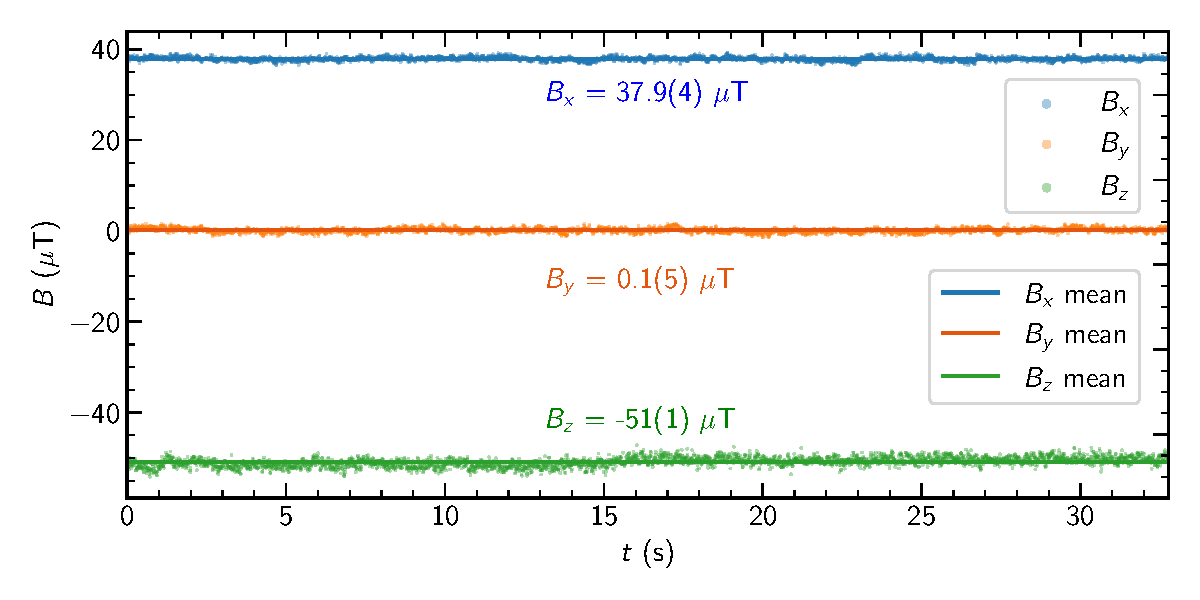
\includegraphics[width=\textwidth]{Versuch6_1}
	\caption{Das gemessene Magnetfeld in die drei kartesischen Raumrichtungen farblich unterscheidbar auf die Zeit aufgetragen. Der Mittelwert der Daten wird als durchgezogene Linie dargestellt.}
	\label{fig:Bmean}
\end{figure}

Es wurde für jede Komponente der Mittelwert gebildet und der Fehler auf die Standardabweichung gesetzt, da dann (per Definition) zwei drittel der Daten innerhalb des \( 1\sigma \) Intervalls liegen. 

Man erhält für die drei kartesischen Komponenten des Erdmagnetfeldes
\begin{equation}\label{eqn:Bxyz}
	B_x = 37.9(4) \unit{\micro T} \qquad B_y = 0.1(5) \unit{\micro T} \qquad B_z = -50.9(1.0) \unit{\micro T}
\end{equation}
. Daraus lässt sich jetzt mit \autoref{eqn:Babs} und \autoref{eqn:theta} die Stärke und Inklination des Erdmagnetfeldes berechnen und man erhält folgende Werte
\begin{equation}\label{eqn:results}
	|\vec{B}| = 63.4(9) \unit{\micro T} \hspace{3cm} \theta = \ang{53.3(6)}
\end{equation}
. Vergleicht man diese Werte mit Literaturwerten \cite{MagCal}
\begin{equation}\label{key}
	|\vec{B}| = 48.40(15) \unit{\micro T} \hspace{3cm} \theta = \ang{63.5(2)}
\end{equation}
erkennt man, dass unsere gemessenen Werte signifikant abweichen. Das liegt wahrscheinlich daran, dass am Versuchsort eine Vielzahl an metallische Objekte vorhanden waren, die Magnetfelder beeinflussen oder sogar selber erzeugen. Der Versuch wurde nämlich in einem Gebäude aus Stahlbeton durchgeführt, in einem Raum voller Elektronik und oberhalb Labore, in welchen Experimente mit elektrischen und Magnetische Felder durchgeführt werden. Es kommt daher zu systematischen Abweichungen, die verringert werden können, indem man die Messung fern von metallischen Objekten wiederholt.

\subsection{Elektromotor}


\begin{center}
	\captionof{table}{Stromrichtung, Drehrichtung und daraus erschlossene Magnetfeldrichtung für die vier Konfigurationen.}
	\begin{tabular}{@{\extracolsep{5mm}} 
			r
			c
			c
			c
		}
		\toprule
		\makecell[t]{Konfiguration}
		&   {\makecell[t]{Stromrichtung}}
		&   {\makecell[t]{Drehrichtung}}
		&   {\makecell[t]{Magnetfeldrichtung}}\\
		\midrule
		1 & \( -\hat{x} \) & \( \circlearrowright \) & \( -\hat{z} \) \\
		2 & \( \phantom{-}\hat{x} \) & \( \circlearrowleft \) & \( -\hat{z} \) \\
		3 & \( -\hat{x} \) & \( \circlearrowleft \) & \( \phantom{-}\hat{z} \) \\
		4 & \( \phantom{-}\hat{x} \) & \( \circlearrowright \) & \( \phantom{-}\hat{z} \) \\
		\bottomrule
	\end{tabular}
	\label{table:1}
\end{center}

\subsection{Stromdurchflossener Leiter}
